\section{Ein allgemeines Resultat: Der Satz von Cauchy-Kovalevskaya}
\label{sec:para2}

Betrachte im Folgenden eine quasilineare PDGL:
\begin{equation} \sum\limits_{|\alpha|=k} a_{\alpha}(D^{k-1} u(x), \dots , Du(x),u(x),x) D^\alpha u(x) + a_0(D^{k-1} u(x),\dots,u(x),x) = 0 \end{equation}
Sei $\Gamma$ eine glatte, orientierte $(n-1)$-dimensionale Hyperfläche im $\RR^n$, $\nu(x) = (\nu_1(x), \dots, \nu_n(x))$ die Einheitsnormale auf $\Gamma$ an $x \in \Gamma$. Sei 
\[\frac{\partial^j u(x)}{\partial \nu^j} = (\nu \cdot \nabla)^j u(x) = \sum\limits_{|\alpha|=j} \frac{j!}{\alpha!} D^\alpha u \cdot \nu^\alpha = \sum\limits_{|\alpha|=j} \frac{j!}{\alpha_1!\cdots\alpha_n!} \frac{\partial^{|\alpha|}u}{\partial x_1^{\alpha_1} \cdots \partial x_n^{\alpha_n}} \nu_1^{\alpha_1} \cdots \nu_n^{\alpha_n}\] die $j$-te Normalenableitung von $u$ an $x$.

\begin{defn}[Cauchy-Problem] \label{def_cauchy_problem}
	Löse die PDGL (1) mit vorgegebenen \Index{Cauchy-Daten} auf $\Gamma$:  \index{Cauchy-Problem}
	\begin{equation}
		u(x) = g_0(x), \frac{\partial u}{\partial \nu} = g_1, \dots, \frac{\partial^{k-1} u}{\partial \nu^{k-1}} = g_{k-1} \end{equation}
\end{defn}

\begin{defn}[analytische Funktion] \label{def_analytische_fkt}
	$f\colon \RR^n \rightarrow \RR$ heißt \Index{analytisch} um $x_0 \in \RR^n$, wenn ein $r > 0$ und $f_\alpha \in \RR$ existiert, sodass
	\[ f(x) = \sum_{\alpha} f_\alpha (x-x_0)^\alpha \]
	für alle $|x-x_0| < r$.
\end{defn}
	
\begin{bem}
	\begin{itemize}
		\item Ist $f$ analytisch um $x_0$, dann ist $f$ unendlich oft stetig differenzierbar um $x_0$, und es gilt $D^\alpha f(x) = f_\alpha \alpha!$. $f$ ist gleich seiner Taylor-Entwicklung auf $|x-x_0| < r$:
		\[ f(x) = \sum_{\alpha} \frac{D^\alpha f(x)}{\alpha!} (x-x_0)^\alpha \]
		\item Eine Hyperfläche $\Gamma$ heißt analytisch um $x_0 \in \Gamma$, wenn es analytische Funktionen $\phi, \psi\colon \RR^n \rightarrow \RR^n$ und ein $r > 0$ gibt mit $\phi = \psi^{-1}, \phi(\Gamma \cap B_r(x_0)) \subset \{x_n = 0\}$.
	\end{itemize}
\end{bem}
	
\begin{thm}[Cauchy-Kovalevskaya] \label{sub:satz_cauchy_kova}
	Seien $\Gamma, g_0,g_1,\dots,g_{k+1},a_\alpha, a_0$ analytisch um $x_0$ mit $\sum\limits_{|\alpha| = k} a_\alpha (D_{k-1},D_{k-2}, \dots,D_0,x) \neq 0$ für alle $x \in \Gamma$ und $D_i \in \RR^{n^i}$. Dann existiert ein $r > 0$ und eine Lösung $u$ zu (1) und (2) auf $B_r(x_0)$. $u$ ist dort analytisch. \index{Cauchy-Kovaleskaya}
\end{thm}

% % % % % % % % % % % % % % % % % % % % % % 11. Apr		
\begin{bem}[Bemerkung]
	\begin{itemize}
		\item Dieser \marginnote{11. Apr}Satz ist das einzig wirkliche allgemeine Resultat in der Theroie der partiellen Differentialgleichungen. 
		\item Der Satz besitzt starke, fast nie gegebene Voraussetzungen (Analytizität)
		\item Der Satz liefert keine Aussage über den Radius $r$: % Bild (2), (3)
			\[ \begin{cases}
				\Delta u = 0 \text{ im } \RR^2 \\
				u = 0 \text{ und } \frac{\partial u}{\partial \nu} = \frac{\varepsilon \delta^2}{x_1^2 + \delta^2} \text{ auf } \Gamma = \{x_2 = 0 \}, \varepsilon,\delta > 0 \end{cases} \]
			$\frac{\varepsilon \delta^2}{x_1^2+\delta}$ ist analytisch und beschränkt durch $\varepsilon$. Eine Lösung ist gegeben durch
			\[ u(x) = -\frac{\varepsilon \delta}{4} \ln \frac{x_1^2 + (x_2 - \delta)^2}{x_1^2+(x_2 + \delta)^2}\]
			$\Rightarrow u$ explodiert um $(0,\delta),(0,-\delta)$, egal, wie klein $\varepsilon$ ist.
		\item \begin{minipage}[t]{11cm}
		$\Gamma$ mit $\sum\limits_{|\alpha| = k} a_\alpha \nu^\alpha \neq 0$ auf $\Gamma$ heißt \Index{nichtcharakteristisch}. In einer PDGL fließt Information entlang so genannter \bet{charakteristischer Kurven}. $\Gamma$ nichtcharakteristisch bedeutet, dass Information quer zu $\Gamma$ fließt. Ein tangentialer Informationsfluss hilft uns nicht. \index{charakteristische Kurve}
		\end{minipage} \hfill
		\begin{minipage}[t][2cm][b]{2.5cm}
		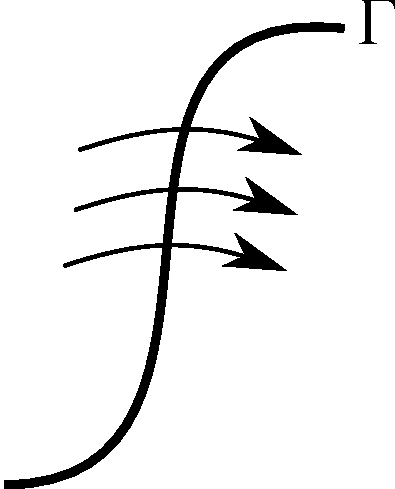
\includegraphics[keepaspectratio,width=2cm]{img/2_charkurv.pdf}
		\end{minipage}
		\textbf{Beispiel:}
		\[ u_t + b \cdot \nabla u = 0 \Leftrightarrow \begin{pmatrix}1 \\ b \end{pmatrix} \cdot \begin{pmatrix}\der u / \der t \\ \der u / \der x_1 \\ \vdots \\ \der u / \der x_1	\end{pmatrix}  = 0 \]
		$\Rightarrow u$ ist konstant entlang der Richtung $\begin{pmatrix}1 \\ b \end{pmatrix}$. \\
		$\Rightarrow$ Anfangsdaten werden entlang charakteristischer Kurven mit Richtung  $\begin{pmatrix}1 \\ b \end{pmatrix}$ transportiert.
		\begin{center}
		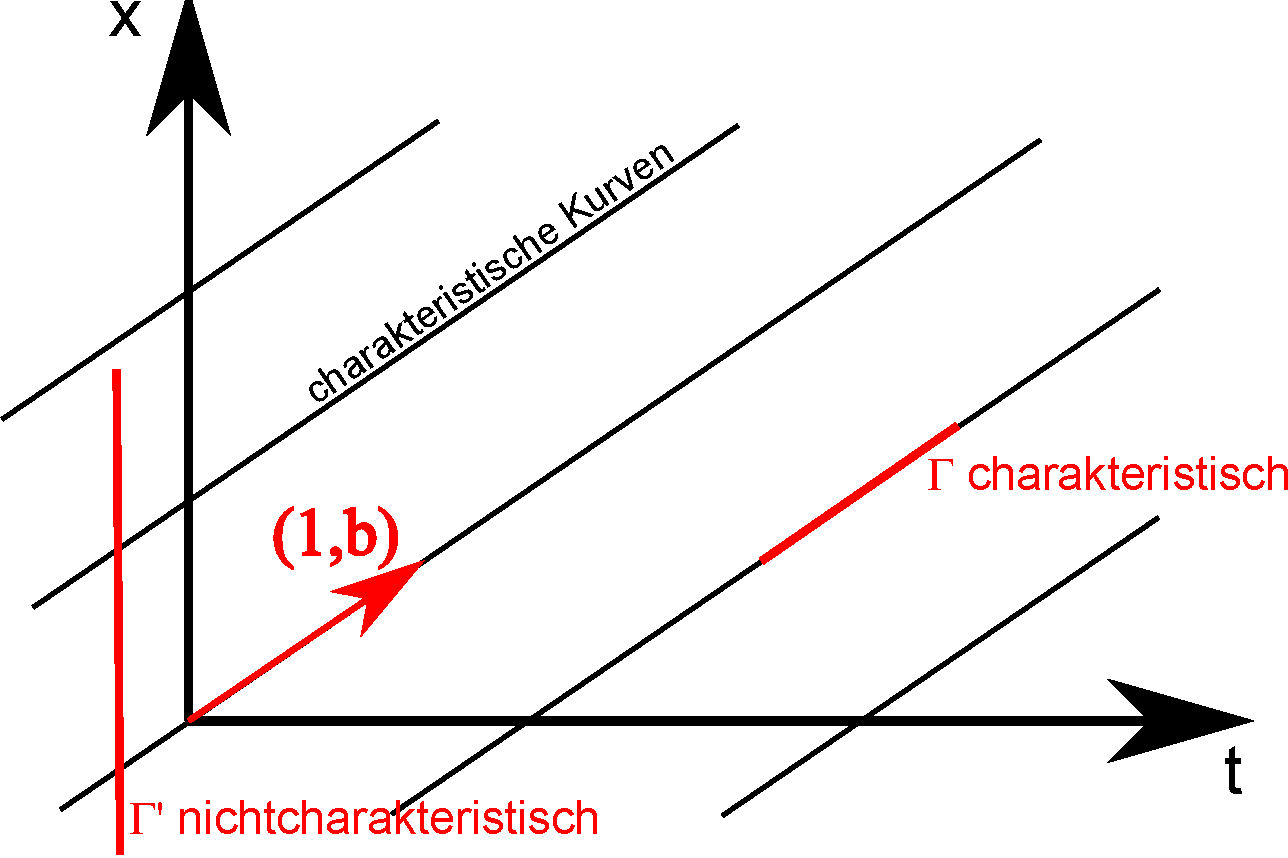
\includegraphics[keepaspectratio, width=7cm]{img/2_bsp_charkurv.pdf}
		\end{center}
	\end{itemize}
\end{bem}
	
\minisec{Beweis}
	Beweisschritte: \begin{enumerate}[(1)]
		\item Reduktion auf $\Gamma = \{ x_n = 0 \}$. \begin{itemize}
			\item Wähle $r, \psi, \phi$ analytisch mit $\psi = \phi^{-1}, \phi(\Gamma \cap B_r(x_0)) \subset \{x_n = 0 \}$. $\Gamma$ ist analytisch auf $B_\rho(x_0)$ mit $\rho \geq r$.
			\item $v(x) = u (\psi (x), u(x) = v (\phi(x))$
			\item $v$ erfüllt die quasilineare PDGL
			\begin{equation}
			 \sum\limits_{|\alpha| = k} b_\alpha(D^{k-1} v(x),\dots,v(x),x) D^\alpha v(x) + b_0(D^{k-1}v(x),\dots,v(x),x)=0 \tag{$*$} \end{equation}
			mit $b_\alpha, b_0$ analytisch und
			\item $b_{(0,\dots,0,k)} \neq 0$ auf $\{x_n = 0\}$, denn:	\marginnote{$\phi_i$: $i$-te Komponente} 
			\[ D^\alpha u = \frac{\der^k v}{\der x_n^k} (D\phi_n)^\alpha + \text{ Terme ohne } \frac{\der^k v}{\der x_n^k} \]
			$\Rightarrow 0 = \sum\limits_{|\alpha|=k} a_\alpha D^\alpha u + a_0 = \underbrace{\enbrace*{ \sum\limits_{|\alpha| = k} a_\alpha (D \phi_n)^\alpha }}_{b_{(0,\dots,0,k)}} \frac{\der^k v}{\der x_n^k} + $ Terme ohne $\frac{\der^k v}{\der x_n^k}$. \\
			$\Rightarrow D\phi_n \parallel \nu$, $\nu = (0,\dots,0,1)$. \marginnote{$\parallel$: parallel} \\
			$\Rightarrow D\phi_n = \kappa \nu, b_{(0,\dots,0,k)} = \kappa^n \sum\limits_{|\alpha|=k} a_\alpha \nu^\alpha \neq 0$ mit einer Konstanten $\kappa$. \end{itemize}
			Wir haben also:
			\[ 0 = \sum\limits_{|\alpha|=k} b_\alpha D^\alpha v + b_0, b_{(0,\dots,0,k)} \neq 0, \quad v(x) = g_0(\psi(x))\]
			\[ \frac{\der v}{\der x_n} = \frac{\der u\circ \psi}{\der x_n} \text{ hängt ab von } g_1,D\psi \]
			\[ \vdots \] \[\frac{\der^{n-1} v}{\der x_n^{k-1}} = \frac{\der^{k-1}(u \circ \psi)}{\der x_n^{k-1}} \text{ hängt ab von } g_1, g_2,\dots,g_{k-1},D\psi,D^2\psi, \dots, D^{k-1} \psi\]
			\[ v(x) =: h_0(x),\quad \frac{\der v}{\der x_n} (x) =: h_1(x),\quad \dots ,\quad \frac{\der^{k-1} v}{\der x_n^{k-1}} =:  h_{k-1}(x) \text{ auf } \Gamma \]
					alles analytisch um 0.			
		\item Ermitte partielle Ableitungen von $v$ auf $\{x_n = 0\}$ (bzw. von $u$ auf $\Gamma$). \\
		1. Ordnung normal: $\frac{\der v}{\der x_n} (0) = h_1(0)$. \\
		1. Ordnung tangential: $\frac{\der v}{\der x_i}(0) = \frac{\der h_0}{\der x_i} (0), i \neq n$ \\
		2. Ordnung: $\frac{\der^2 v}{\der x_n^2} (0) = h_2(0)$ \\
		$\frac{\der^2 v}{\der x_n \der x_i} (0) = \frac{\der h_1}{\der x_i} (0), i \neq n$ \\
		$\frac{\der^2 v}{\der x_i \der x_j} (0) = \frac{\der^2 h_0}{\der x_i \der x_j} (0), i,j \neq n$ \\
		$j$. Ordnung: $D^\alpha v = \frac{\der^{|\alpha|-\alpha_n} h_{\alpha_n}}{\der x^{\alpha'}}$ mit $\alpha' = (\alpha_1,\dots,\alpha_{n-1},0)$ für $j < k$ \\
		$k$. Ordnung: analog zu $j$, außer
		\[ \frac{\der^k v}{\der x_n^k} = -\frac{1}{b_{(0,\dots,0,k)}} \left[ \sum\limits_{\substack{|\alpha|=k \\ \alpha \neq (0,\dots,0,k)}} b_\alpha D^\alpha v + b_0 \right] =: h_k \]
		höhere Ordnung: analog zu $k$, nur dieses Mal benutze $\frac{\der^{(\alpha_n-k)}}{\der x_n^{\alpha_n-k}}$ $(*)$.
		$\Rightarrow h$ Normalenableitungen auf der nichtcharakteristischen Hyperfläche legen alle partiellen Ableitungen auf der Fläche fest.
% % % % % % % % % % % % % 15. Apr.
		\item Zeige Konvergenz der Taylor-Entwicklung von $v$ um $x=0$ (bzw. von $u$ um $x_0$).\marginnote{15. Apr} Die geht einfacher bei 1.-Ordnungs-Systemen:
		\begin{itemize}
			\item o.B.d.A. sind $h_0,h_1,\dots,h_{k-1} = 0$ (ansonsten subtrahiere eine geeignete analytische Funktion von $v$)
			\item transformiere in 1. Ordnungs-System
			\[ w := \enbrace*{v, \frac{\der v}{\der x_1},\dots,\frac{\der v}{\der x_n}, \frac{\der^2 v}{\der x_1^2}, \dots, \frac{\der^{k-1} v}{\der x_n^{k-1}}}: \RR^n \longrightarrow \RR^m \]
			\begin{equation} \Rightarrow \begin{cases}
				w_{x_n} = \sum\limits_{j=1}^{n-1} \underbrace{B_j(w,x)}_{\in \RR^{n \times m}} w_{x_j} + \underbrace{c(w,x)}_{\in \RR^m} \\
				w = 0 \text{ auf } \Gamma
			\end{cases} \tag{$*$} \end{equation}
			$B_j$ und $c$ sind analytisch, d.h.
			\[ B_j(z,x) = \sum\limits_{\gamma,\delta} B_{j\gamma\delta} z^\gamma x^\delta, \qquad c(z,x) = \sum\limits_{\gamma,\delta} c_{\gamma \delta} z^\gamma x^\delta \]
			mit einem Konvergenzradius $R$, d.h. $|x^2+|z^2| < R^2$.
			\item o.B.d.A. sind $B_j$ und $c$ unabhängig von $x_n$ (ansonsten füge weitere Komponente $w^{m+1}$ zu $w$ hinzu mit $w^{m+1} = x_n$, d.h. $w_{x_n}^{m+1} = 1$ als zusätzliche Zeile in $(*)$.)
			\item Potenzreihenansatz: $w = \sum\limits_{\alpha} w_\alpha x^\alpha$.
			\item Drücke $w_\alpha$ aus in Termen der $B_{j\gamma\delta}, c_{\gamma\delta}$:
				\begin{itemize}
					\item $\alpha_n = 0$:
					\[ w_\alpha = \frac{D^\alpha w(0)}{\alpha_1! \cdots \alpha_n!} = 0, \]
					da $w = 0$ auf $\{x_n = 0\}$.
					\item $\alpha_n = 1$: PDGL $(*)$:
					\begin{equation}
					\begin{aligned}
						w_{x_nx_i} &= \sum\limits_{j=1}^{n-1} \enbrace*{B_j(w,x) w_{x_jx_i} + B_{j,x_i}(w,x) w_{x_j} + \sum\limits_{p=1}^{m} B_{j,w^p} (w,x) w_{x_i}^p w_{x_j}} \\
						&+ c_{x_i}(w,x) + \sum\limits_{p=1}^{m} c_{w^p} (w,x) w_{x_i}^p \\ \notag
						&= c_{x_i} (w,x) \text{ für } i \neq n, \quad \text{da } w_{x_jx_i} = 0, w_p = 0
					\end{aligned}
					\end{equation}
					\[ \Rightarrow w_\alpha = \frac{D^\alpha w(0)}{\alpha_1! \cdots \alpha_n!} = \frac{D^{\alpha'} c(\overbrace{w(0)}^{=0},0)}{\alpha_1! \cdots \alpha_n!} \text{ mit } \alpha = \begin{pmatrix} \alpha_1 \\ \vdots \\ \alpha_{n-1} \\ 1 \end{pmatrix}, \alpha' = \begin{pmatrix} \alpha_1 \\ \vdots \\ \alpha_{n-1} \\ 0 \end{pmatrix} \]
					\item allgemeines $\alpha$:
					\begin{equation}
					\begin{aligned}
						D^\alpha w = D^{\alpha'} \frac{\der \alpha_n}{\der x_1^{\alpha_n}} w = D^{\alpha'} \frac{\der^{\alpha_n-1}}{\der x_n^{a_n -1}} w_{x_n} &\overset{(*)}{=} \widetilde{P}_\alpha (\dots,D_z^\gamma D_x^\delta B_j,\dots,D_z^\gamma D_x^\delta c,\dots D^\beta w,\dots) \\ \notag
						&= P_\alpha(\dots,B_{j\gamma\delta},\dots,c_{\gamma \delta},\dots,w_\beta,\dots)
					\end{aligned}
					\end{equation}
					für ein Polynom $P_\alpha$ mit nicht negativen Koeffizienten und $\beta_n \leq \alpha_n -1$ für alle Multiindizes $\beta$ in den Argumenten
					\[ w_\alpha = \frac{D^\alpha w}{\alpha!} = \frac{1}{\alpha_1! \cdots \alpha_n!} P_\alpha( \cdots ) \]
					\item Wähle $K > 0$ groß genug und $s \leq \frac{R}{\sqrt{m+n}}$ mit $R$ Konvergenzradius von $B_j,c$, sodass
					\[ | B_{j \gamma \delta}|,|c_{\gamma \delta}| < \frac{K |\alpha|!}{\alpha_1! \cdots \alpha_n! s^{|\alpha|}} \]
					Dies ist möglich, da für $\sqrt{z^2+x^2} < R$ gilt: $|B_{j \gamma \delta} z^\gamma x^\delta|,|c_{\gamma \delta} z^\gamma x^\delta| \leq K$ für ein $K > 0 \Rightarrow |B_{j \gamma \delta}|,|c_{\gamma \delta}| \leq \frac{K}{z^\gamma x^\delta} \leq \frac{K}{s^{|\alpha|}} \leq \frac{K |\alpha|!}{\alpha! s^{|\alpha|}}$.
					Definiere:
					\[B_j^* := \frac{Ks}{s-(x_1+\dots+x_{n-1})-(z_1 + \dots + z_n)} \begin{pmatrix} 1 & \dots & 1 \\ \vdots & \ddots & \vdots \\ 1 & \dots & 1	\end{pmatrix} = K \sum\limits_{\alpha \in \NN_0^{m+n-1}} \frac{|\alpha|!}{\alpha! \cdot s^{|\alpha|}} \begin{pmatrix} 1 & \dots & 1 \\ \vdots & \ddots & \vdots \\ 1 & \dots & 1	\end{pmatrix} \]
					\[ c^* := \frac{Ks}{s-(x_1 + \dots + x_{n+1}) + (z_1 + \dots + z_n)} \begin{pmatrix}
					1 \\ \vdots \\ 1 \end{pmatrix} = K \sum\limits_{\alpha \in \NN_0^{m+n-1}} \frac{|\alpha|!}{\alpha! \cdot s^{|\alpha|}} \begin{pmatrix} 1 \\ \vdots \\ 1 \end{pmatrix} \]
					 $B_j^*, c^*$ sind analytisch und haben Konvergenzradius $\frac{s}{\sqrt{m+n}}$.
					 \item Betrachte $w_{x_n}^* = \sum\limits_{j=1}^{n-1} B_j^*(w^*,x) w_{x_j}^* + c^*(w^*,x)$ mit $w^* = 0$ auf $\{x_n = 0\}$. Dies hat die Lösung
					 \[ w^*(x) = \frac{1}{mn} (s-(x_1 + \dots + x_{n-1})) - \sqrt{(s-(x_1+\dots+x_{n-1}))^2-2mnKsx_n} \cdot \begin{pmatrix}	1 \\ \vdots \\ 1 \end{pmatrix}\]
					 $w^*$ ist analytisch für $|x|<r$ mit $r$ klein genug, d.h. $w^*  =\sum\limits_{\alpha} w_\alpha^* x^\alpha$.
					 \begin{equation}
					 \begin{aligned}
					 	|w_\alpha^k| &= \frac{1}{\alpha!} P_\alpha(\dots,B_{j\gamma\delta},\dots,c_{\gamma\delta},\dots,w_\beta,\dots) \\ \notag
					 	&\leq \frac{1}{\alpha!}  P_\alpha(\dots,|B_{j\gamma\delta}|,\dots,|c_{\gamma\delta}|,\dots,|w_\beta|,\dots) \text{, da Koeffizienten nicht negativ} \\
					 	&\leq \frac{1}{\alpha} P_\alpha (\dots,B_{j\gamma\delta}^*, \dots, c_{\gamma \delta}^*,\dots, w_\beta^*,\dots) \\
					 	&= (w_\alpha^*)^k \text{ per Induktion, da } \beta_n \leq \alpha_n - 1
					 \end{aligned}
					 \end{equation}
					 $\Rightarrow w^*$ majorisiert $w(x) = \sum_{\alpha} w_\alpha x^\alpha$. \\
					 $\Rightarrow$ auch $\sum\limits_{\alpha} w_\alpha x^\alpha$ konvergiert um 0. \qed
				\end{itemize}
		\end{itemize}
	\end{enumerate}
	
\begin{bsp} \label{bsp_1}
	Die PDGL $u_{x_1} + u_{x_2} = 1$ \marginnote{[1]} hat die allgemeine Lösung $u = \frac{x_1+x_2}{2} + F(x_1-x_2)$ für $F\colon \RR \rightarrow \RR$ beliebig. \begin{itemize}
	\item \[ \left. \begin{cases}
		u_{x_1} + u_{x_2} = 1 \\
		u = 0 \text{ auf } \Gamma = \{x_1 = -x_2\} \end{cases} \right\} \Rightarrow u(\alpha,-\alpha) = F(2\alpha) = 0 \Rightarrow F \equiv 0 \]
	\[ \nu = \frac{1}{\sqrt{2}} \begin{pmatrix} 1 \\ 1 \end{pmatrix}, \sum\limits_{|\alpha| = 1} a_\alpha \nu^\alpha = a_{(1,0)} \nu_1^1 \nu_2^0 + a_{(0,1)} \nu_1^0 \nu_2^1 = \nu_1 + \nu_2 = \sqrt{2} \neq 0 \]
	Also ist $\Gamma$ nichtcharakteristisch.
	\item \[ \left. \begin{cases}
		u_{x_1} + u_{x_2} = 1 \\
		u = 0 \text{ auf } \Gamma = \{x_1 = x_2\} \end{cases} \right\} \Rightarrow u(\alpha,\alpha) = \alpha + F(0) = 0 \Rightarrow \lightning  \]
	\[ \nu = \frac{1}{\sqrt{2}} \begin{pmatrix} 1 \\ -1 \end{pmatrix}, \sum\limits_{|\alpha| = 1} a_\alpha \nu^\alpha = \nu_1 + \nu_2 = 0 \]
	Also ist $\Gamma$ charakteristisch.
	\item \[ \left. \begin{cases}
		u_{x_1} + u_{x_2} = 1 \\
		u = x_1 \text{ auf } \Gamma = \{x_1 = x_2\} \end{cases} \right\} \Rightarrow u(\alpha,\alpha) = \alpha + F(0) = \alpha \Rightarrow F(0)=0 \Rightarrow \text{ unendlich viele Lösungen} \]
	\end{itemize}
\end{bsp}
\newpage
		